% LUTGPT --- short walkthrough deck (companion to lutgpt_research_report.tex).
% 16:9 beamer, default theme, no navigation clutter.

\documentclass[aspectratio=169]{beamer}
\usetheme{default}
\setbeamertemplate{navigation symbols}{}
\setbeamertemplate{footline}[frame number]

\usepackage{tikz}
\usetikzlibrary{arrows.meta,positioning,calc,fit,backgrounds,shapes}
\usepackage{amsmath,amssymb,booktabs,xcolor,array}
\usepackage[T1]{fontenc}

\newcommand{\R}{\mathbb{R}}
\newcommand{\bstar}{b^{*}}
\newcommand{\jstar}{j^{*}}
\newcommand{\Tsoft}{T_{\mathrm{soft}}}
\newcommand{\Tsel}{T_{\mathrm{sel}}}
\newcommand{\dout}{d_{\mathrm{out}}}
\newcommand{\dv}{d_{v}}
\newcommand{\softmax}{\operatorname{softmax}}
\newcommand{\sign}{\operatorname{sign}}
\newcommand{\dqk}{d_{qk}}
\newcommand{\bp}{\mathbf{b}}

\setlength{\leftmargini}{1.2em}
\setlength{\leftmarginii}{1em}

\title{LUTGPT --- a walkthrough}
\author{Anatoly Starostin}
\date{}

\setbeamerfont{frametitle}{size=\large,series=\bfseries}
\setbeamerfont{block title}{size=\small,series=\bfseries}

\begin{document}

% =====================================================================
\frame{\titlepage}

% =====================================================================
\begin{frame}{Roadmap}
\begin{enumerate}
\item The LUT primitive \texttt{MultiHeadLut}: math, hyperparameters
\item Two forward modes: \texttt{hard} vs \texttt{hybrid\_smooth}
\item Backward pass: weight grad matches forward, input grad is soft
\item Ranking vs.\ standard (Euclidean) embeddings
\item The LUT transformer block
\item Dual residual stream (E-stream, D-stream)
\item Final architecture: vanilla baseline vs.\ LUTGPT
\item The five LUTs and their roles at the interfaces
\item Experiments: matched-budget loss numbers, validation curves
\item Appendix: the soft-surrogate backward, derived
\end{enumerate}
\end{frame}

% =====================================================================
\begin{frame}{\texttt{MultiHeadLut}: the LUT primitive}

\textbf{Signature.} \hspace{0.5em}
\(F : \R^{E} \to \R^{H \times \dout}, \quad x \mapsto y_h = \displaystyle\sum_{s=1}^{\mathrm{tph}} \mathrm{Lut}_{h,s}(x).\)

\medskip
\begin{columns}[T,onlytextwidth]
\begin{column}{0.46\textwidth}
\textbf{Hyperparameters:}
\begin{itemize}
\item \(E\): input width
\item \(\dout\): output width per head
\item \(H\): number of heads
\item \(\mathrm{tph}\): tables per head
\item \(N\) = NAP: anchor pairs per table
\item \(K = 2^N\): rows per table
\end{itemize}

\medskip
\textbf{Per layer:} \(H \cdot \mathrm{tph}\) independent tables, each of shape \(K \times \dout\).
\end{column}
\begin{column}{0.52\textwidth}
\textbf{One table \(\mathrm{Lut}_{h,s}\):}
\begin{enumerate}
\item Fix \(N\) anchor pairs \((a_j, b_j)\) at construction.
\item Compute \(N\) bits: \(\beta_j = [x_{a_j} > x_{b_j}] \in \{0, 1\}.\)
\item Pack into one index: \(\mathrm{idx} = \sum_{j=1}^{N} 2^{N-j}\, \beta_j \in \{0, \dots, K{-}1\}.\)
\item Look up row: \(y = W[\mathrm{idx}],\quad W \in \R^{K \times \dout}.\)
\end{enumerate}

\medskip
\textbf{Per-head output:} sum of \(\mathrm{tph}\) such row lookups.
\end{column}
\end{columns}

\vspace{0.6em}
\hrule
\vspace{0.4em}
\small\emph{The forward is a comparison + bit-pack + row gather --- no dot products, no nonlinear activations.}
\end{frame}

% =====================================================================
\begin{frame}{Two forward modes: \texttt{hard} vs \texttt{hybrid\_smooth}}

Let \(d_j = x_{a_j} - x_{b_j}\) and \(\bstar = ([d_j > 0])_{j=1}^{N}\) (the sign-pack index).

\smallskip
\begin{columns}[T,onlytextwidth]
\begin{column}{0.5\textwidth}
\textbf{\texttt{hard}} --- inference default
\[ \boxed{\;y^{\mathrm{hard}} = W[\bstar]\;} \]
\begin{itemize}
\item \(O(N)\) comparisons + 1 row gather.
\item No softmax, no temperatures, no row blend.
\item This is the operation a rank-coded sparse-lookup accelerator would execute.
\end{itemize}
\end{column}
\begin{column}{0.5\textwidth}
\textbf{\texttt{hybrid\_smooth}} --- training default
\[ \boxed{\;y^{\mathrm{hyb}} = (1{-}u)\, W[\bstar] + u\, W[b_{\mathrm{alt}}]\;} \]
\begin{itemize}
\item \(b_{\mathrm{alt}}\): flip the bit at \(\jstar = \arg\min_j |d_j|\).
\item \(u = \sigma(-\Delta/\Tsel) \in (0, \tfrac{1}{2}]\) with \(\Delta = 2|d_{\jstar}|/(\Tsoft + |d_{\jstar}|).\)
\item As confidence \(\uparrow\), \(u \to 0\); hybrid \(\to\) hard.
\end{itemize}
\end{column}
\end{columns}

\vspace{0.5em}
\small\emph{Hybrid-smooth is a two-row blend of the hard pick and its closest neighbour --- one extra row gather, no \(K\)-wide softmax.}
\end{frame}

% =====================================================================
\begin{frame}{Backward pass: weight grad matches forward, input grad is soft}

The forward is sparse (1 or 2 rows). The backward is \emph{asymmetric}.

\medskip
\begin{columns}[T,onlytextwidth]
\begin{column}{0.5\textwidth}
\textbf{(A) Weight gradient --- matches the forward.}
\begin{itemize}
\item \texttt{hard}: scatter \(g = \partial L/\partial y\) into one row \(\bstar\).
\item \texttt{hybrid\_smooth}: scatter \((1{-}u)\, g\) into \(\bstar\), \(u\, g\) into \(b_{\mathrm{alt}}\).
\item Honest derivative of the truncated forward: no phantom update on rows the forward did not touch.
\end{itemize}
\end{column}
\begin{column}{0.5\textwidth}
\textbf{(B) Input + temperature gradient --- soft surrogate over all \(K\) rows.}
\begin{itemize}
\item Backprop \emph{as if} the forward had been the full-K soft mode
\[ y_{\mathrm{full}} = \sum_{b} \pi(b)\, W[b], \quad \pi = \softmax(\mathcal{S}/\Tsel). \]
\item Every anchor pair gets a non-zero derivative each step.
\item Same regardless of which forward mode actually ran.
\end{itemize}
\end{column}
\end{columns}

\medskip
\hrule
\vspace{0.4em}
\small\emph{Why the asymmetry?} The literal Jacobian of \(\bstar\) w.r.t.\ \(x\) is zero almost everywhere (the forward is piecewise constant). The full-K surrogate restores a dense gradient on \(x\) without lying about which weights were used. \textbf{Full derivation in the appendix.}
\end{frame}

% =====================================================================
\begin{frame}{Ranking vs.\ standard (Euclidean) embeddings}

\begin{columns}[T,onlytextwidth]
\begin{column}{0.49\textwidth}
\textbf{Linear projection} \( y = W x \)
\begin{itemize}
\item Interprets \(x\) as a Euclidean vector.
\item \(y_k = \sum_i W_{ki}\, x_i\) --- a weighted sum.
\item Linear in \(x\): scales with \(\|x\|\).
\item Output a smooth function of \(x\).
\end{itemize}
\end{column}
\begin{column}{0.49\textwidth}
\textbf{LUT} \( y = W[\mathrm{idx}(x)] \)
\begin{itemize}
\item Interprets \(x\) by the \emph{ordering} of its coordinates (which dominates which at the chosen pairs).
\item Output independent of \(\|x\|\); a sign-pack is scale-invariant.
\item Nonlinear and piecewise constant in \(x\) --- the row jumps when an anchor flips.
\end{itemize}
\end{column}
\end{columns}

\vspace{0.8em}
\hrule
\vspace{0.5em}
\textbf{Closest deep-learning analogue: 2-layer MLP with widening + ReLU.}

\medskip
\begin{itemize}
\item MLP: expand \(\R^E \to \R^{4E}\) (the hidden layer), apply a piecewise-linear nonlinearity, project back. Sparsely \emph{activates} a subset of the \(4E\) hidden units that depend on \(x\).
\item LUT: expand \(\R^E \to \R^{K}\) of candidate rows (\(K = 2^N\) typically \(\gg E\)), select \emph{exactly one row} as a function of \(x\)'s sign pattern, project that row into \(\R^{\dout}\).
\item Both: \textbf{widen, sparsely activate, project down}. LUT is much sparser (one row vs.\ many active hidden units).
\end{itemize}
\end{frame}

% =====================================================================
\begin{frame}{The LUT transformer block}

\begin{columns}[T,onlytextwidth]
\begin{column}{0.49\textwidth}
\textbf{Vanilla transformer block}
\begin{itemize}
\item LayerNorm \(\to\) Q, K, V Linear \(\to\) SDPA \(\to\) out\_proj Linear \(\to\) \texttt{+ residual}
\item LayerNorm \(\to\) FFN (Linear \(D{\to}4D\), GELU, Linear \(4D{\to}D\)) \(\to\) \texttt{+ residual}
\end{itemize}

\medskip
Two sub-blocks, two residual adds per layer.
\end{column}
\begin{column}{0.49\textwidth}
\textbf{LUT block}
\begin{itemize}
\item MeanAbsNorm \(\to\) \texttt{qk\_lut}, \texttt{v\_lut} \(\to\) SDPA (RoPE on Q, K) \(\to\) \texttt{out\_proj\_lut} \(\to\) \texttt{+ residual}
\item \textbf{No separate FFN.}
\end{itemize}

\medskip
One sub-block per layer. \texttt{out\_proj\_lut} is the widest piece in the block (NAP = 7, tph = 512) and plays the combined role of vanilla's out\_proj + FFN.
\end{column}
\end{columns}

\vspace{0.8em}
\hrule
\vspace{0.4em}
\small\emph{Why no FFN?} A standalone LUT is already a wide, sparsely-activated nonlinearity (see previous slide). The block-level expansion that vanilla buys via \texttt{out\_proj + FFN} is bought here by sizing \texttt{out\_proj\_lut} generously.
\end{frame}

% =====================================================================
\begin{frame}{Dual residual stream}

\textbf{Why not LUT everywhere?} A LUT unembedder \(\R^{E} \to \R^{|V|}\) at \(|V| = 32{,}768\) would dominate the model, and the rank-coded representation is the wrong input for a cross-entropy loss that wants magnitude-coded logits.

\medskip
\textbf{Solution: split the residual stream.}

\begin{columns}[T,onlytextwidth]
\begin{column}{0.5\textwidth}
\textbf{E-stream} (width \(E\), rank-coded backbone)
\begin{itemize}
\item Fed by \texttt{tok\_emb}.
\item Read by every per-layer LUT.
\item Mutated only by per-layer \texttt{out\_proj\_lut}.
\end{itemize}
\end{column}
\begin{column}{0.5\textwidth}
\textbf{D-stream} (width \(D\), Euclidean accumulator)
\begin{itemize}
\item Initialised to \(0\).
\item Written by an ``adapter'': one \texttt{emb\_resid\_lut} at the embedding, plus one \texttt{residual\_lut} per layer.
\item Read once by the dense linear unembedder.
\end{itemize}
\end{column}
\end{columns}

\vspace{0.5em}
\small\emph{The LUT adapter projects rank-coded embeddings back to Euclidean geometry, so the dense unembedder sees a familiar input. The E-stream can be made narrow (\(E = 192\)) while the D-stream stays at unembedder width (\(D = 384\)) --- the asymmetric backbone of \texttt{exp755}.}
\end{frame}

% =====================================================================
\begin{frame}[fragile]{Final architecture: vanilla vs.\ LUTGPT}
\vspace{-0.5em}
\begin{columns}[T,onlytextwidth]
\begin{column}{0.32\textwidth}
\centering
\textbf{Vanilla baseline}

\medskip
\resizebox{\linewidth}{!}{%
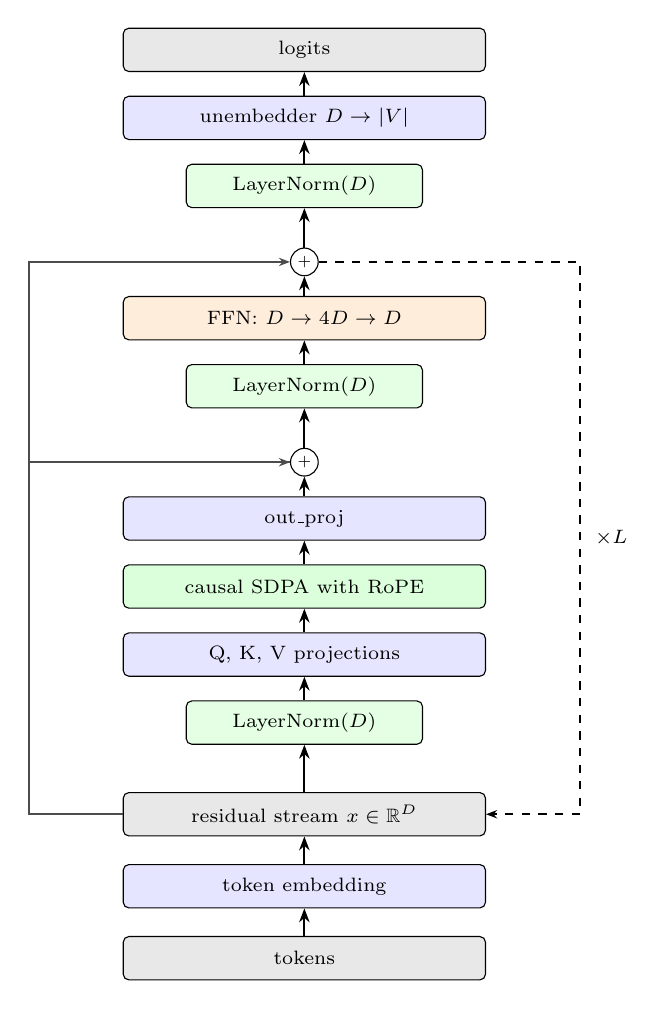
\begin{tikzpicture}[
    every node/.style={font=\scriptsize},
    box/.style={rectangle, draw, rounded corners=2pt, align=center, inner sep=4pt, fill=#1, minimum height=0.55cm, minimum width=4.6cm},
    box/.default=blue!8,
    proj/.style={box=blue!10},
    norm/.style={box=green!10, minimum width=3cm},
    op/.style={box=green!14, minimum width=4.6cm},
    ff/.style={box=orange!14, minimum width=4.6cm},
    stream/.style={box=gray!18, minimum width=4.6cm},
    arr/.style={-{Stealth[length=5pt]}, thick},
    add/.style={circle, draw, inner sep=1.2pt, fill=white, font=\tiny},
    sidearr/.style={-{Stealth[length=4pt]}, thick, gray!60!black},
]
\node[stream] (tokens) at (0, 0) {tokens};
\node[proj, above=0.35cm of tokens] (emb) {token embedding};
\node[stream, above=0.35cm of emb] (xres) {residual stream $x \in \mathbb{R}^D$};
\node[norm, above=0.6cm of xres] (ln1) {LayerNorm($D$)};
\node[proj, above=0.3cm of ln1] (qkv) {Q, K, V projections};
\node[op, above=0.3cm of qkv] (sdpa1) {causal SDPA with RoPE};
\node[proj, above=0.3cm of sdpa1] (oproj) {out\_proj};
\node[add, above=0.25cm of oproj] (a1) {$+$};
\node[norm, above=0.5cm of a1] (ln2) {LayerNorm($D$)};
\node[ff, above=0.3cm of ln2] (ff) {FFN: $D \to 4D \to D$};
\node[add, above=0.25cm of ff] (a2) {$+$};
\node[norm, above=0.5cm of a2] (lnf) {LayerNorm($D$)};
\node[proj, above=0.3cm of lnf] (head) {unembedder $D \to |V|$};
\node[stream, above=0.3cm of head] (logits) {logits};
\draw[arr] (tokens) -- (emb); \draw[arr] (emb) -- (xres);
\draw[arr] (xres) -- (ln1); \draw[arr] (ln1) -- (qkv);
\draw[arr] (qkv) -- (sdpa1); \draw[arr] (sdpa1) -- (oproj);
\draw[arr] (oproj) -- (a1); \draw[arr] (a1) -- (ln2);
\draw[arr] (ln2) -- (ff); \draw[arr] (ff) -- (a2);
\draw[arr] (a2) -- (lnf); \draw[arr] (lnf) -- (head);
\draw[arr] (head) -- (logits);
\coordinate (leftrail) at (-3.5, 0);
\draw[sidearr] (xres.west) -- (xres.west -| leftrail) -- (a1.west -| leftrail) -- (a1.west);
\draw[sidearr] (a1.west)   -- (a1.west -| leftrail)   -- (a2.west -| leftrail) -- (a2.west);
\coordinate (rrail) at (3.5, 0);
\draw[dashed, black, -{Stealth[length=4pt]}, line width=0.6pt]
    (a2.east) -- (a2.east -| rrail) -- (xres.east -| rrail) -- (xres.east);
\node[anchor=west, fill=white, inner sep=1pt, font=\scriptsize] at ($(a2.east -| rrail)!0.5!(xres.east -| rrail) + (0.15,0)$) {$\times L$};
\end{tikzpicture}%
}
\end{column}
\begin{column}{0.65\textwidth}
\centering
\textbf{LUTGPT}

\medskip
\resizebox{\linewidth}{!}{%
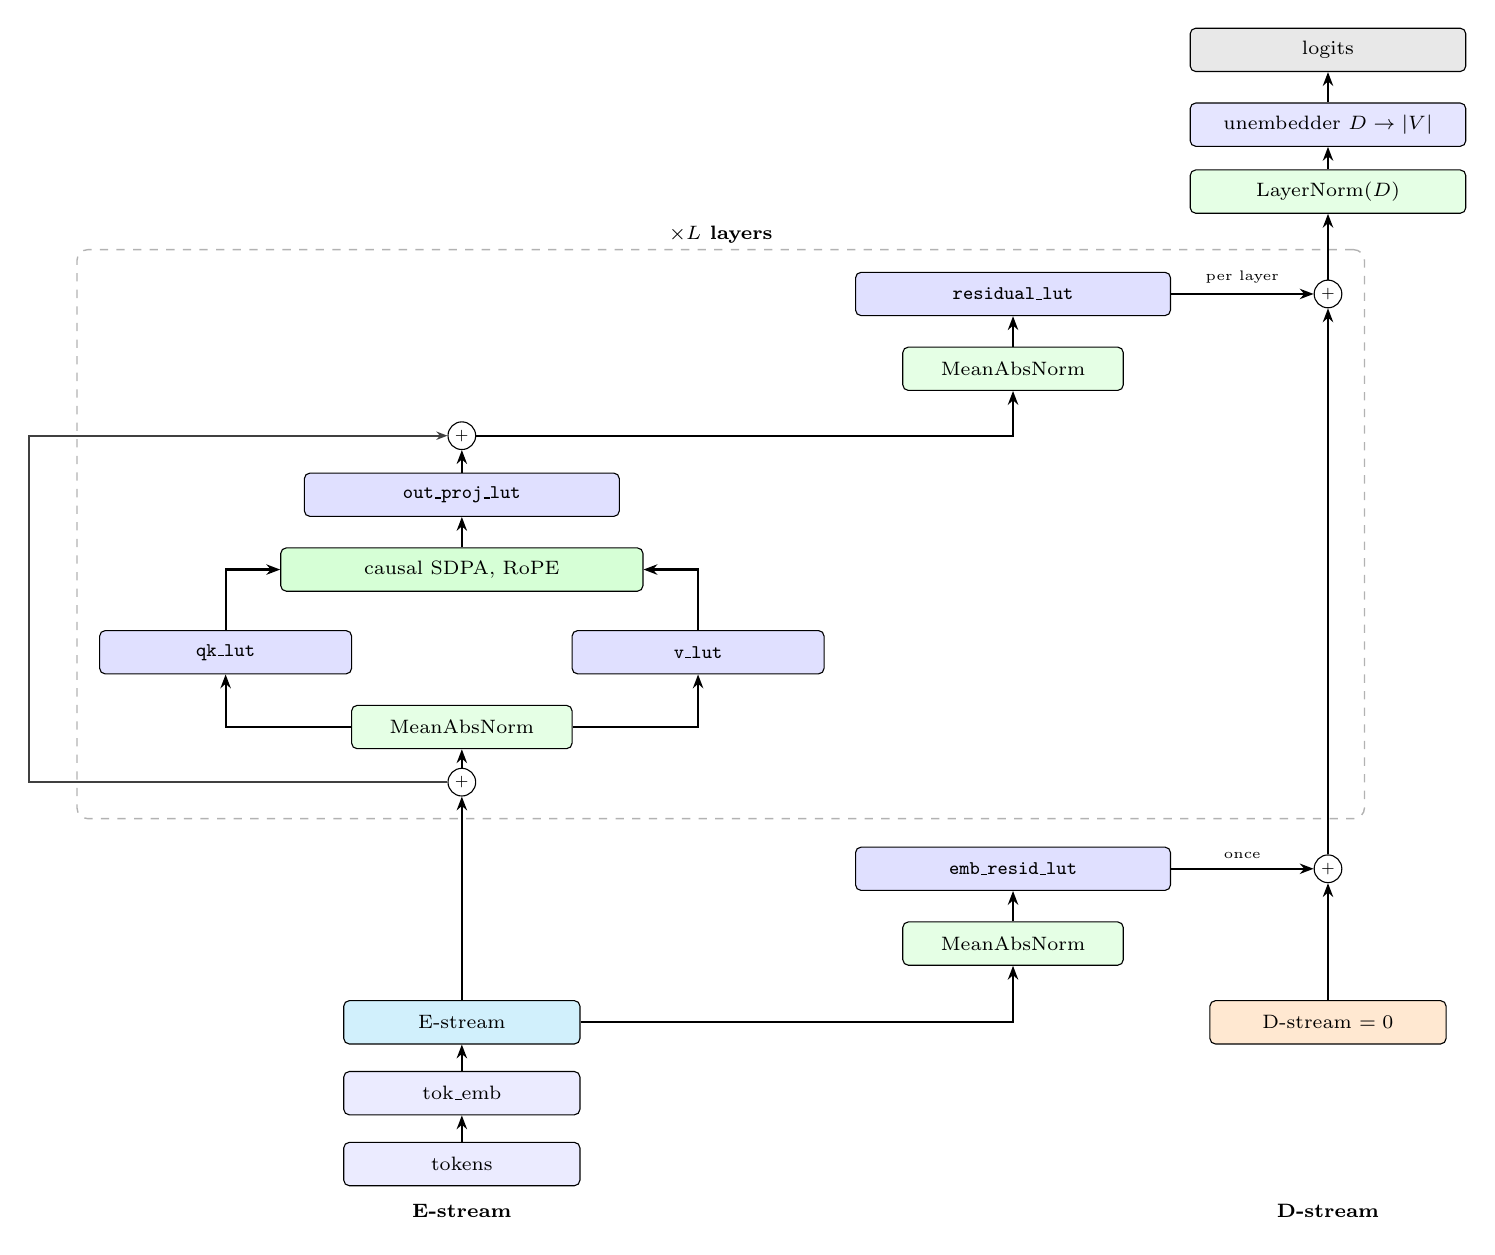
\begin{tikzpicture}[
    every node/.style={font=\scriptsize},
    box/.style={rectangle, draw, rounded corners=2pt, align=center, inner sep=4pt, fill=#1, minimum height=0.55cm},
    box/.default=blue!8,
    lut/.style={box=blue!12, minimum width=4.0cm},
    norm/.style={box=green!10, minimum width=2.8cm},
    op/.style={box=green!16, minimum width=4.6cm},
    emb/.style={box=blue!8, minimum width=3cm},
    estr/.style={box=cyan!18, minimum width=3cm},
    dstr/.style={box=orange!18, minimum width=3cm},
    final/.style={box=gray!14, minimum width=3cm},
    arr/.style={-{Stealth[length=5pt]}, thick},
    sidearr/.style={-{Stealth[length=4pt]}, thick, gray!50!black},
    add/.style={circle, draw, inner sep=1.2pt, fill=white, font=\tiny},
    streamlabel/.style={font=\scriptsize\bfseries, anchor=south},
]
% --- E-stream column (x = 0) ----------------------------------------
\node[emb]  (tokens)  at (0,  0.0)  {tokens};
\node[emb]  (tokemb)  at (0,  0.9)  {tok\_emb};
\node[estr] (xE0)     at (0,  1.8)  {E-stream};
\node[add]  (aEin)    at (0,  4.85) {$+$};
\node[norm] (mn1)     at (0,  5.55) {MeanAbsNorm};
\node[lut, minimum width=3.2cm] (qklut) at (-3.0, 6.5) {\texttt{qk\_lut}};
\node[lut, minimum width=3.2cm] (vlut)  at ( 3.0, 6.5) {\texttt{v\_lut}};
\node[op]   (sdpa)    at (0,  7.55) {causal SDPA, RoPE};
\node[lut]  (op2)     at (0,  8.5)  {\texttt{out\_proj\_lut}};
\node[add]  (aE)      at (0,  9.25) {$+$};

% --- Adapter column (x = 7) -----------------------------------------
% Residual adapters live to the right of the E-stream; they read from
% the E-stream and write to the D-stream. This mirrors how vanilla's
% attention + FFN sub-blocks both live in the residual-stream column.
\node[norm] (mn0)     at (7,  2.8)  {MeanAbsNorm};
\node[lut]  (embres)  at (7,  3.75) {\texttt{emb\_resid\_lut}};
\node[norm] (mn2)     at (7, 10.1)  {MeanAbsNorm};
\node[lut]  (reslut)  at (7, 11.05) {\texttt{residual\_lut}};

% --- D-stream column (x = 11) ---------------------------------------
\node[dstr] (xD0)     at (11, 1.8)  {D-stream $= 0$};
\node[add]  (aD0)     at (11, 3.75) {$+$};
\node[add]  (aD1)     at (11,11.05) {$+$};
\node[box=green!10, minimum width=3.5cm, rounded corners=2pt, draw,
      align=center, inner sep=4pt] (lnf)   at (11, 12.35) {LayerNorm($D$)};
\node[box=blue!10,  minimum width=3.5cm, rounded corners=2pt, draw,
      align=center, inner sep=4pt] (head)  at (11, 13.2)  {unembedder $D \to |V|$};
\node[box=gray!18,  minimum width=3.5cm, rounded corners=2pt, draw,
      align=center, inner sep=4pt] (logits)at (11, 14.15) {logits};

% --- E-stream main flow (straight up, x=0) --------------------------
\draw[arr] (tokens) -- (tokemb);
\draw[arr] (tokemb) -- (xE0);
\draw[arr] (xE0)    -- (aEin);
\draw[arr] (aEin)   -- (mn1);
\draw[arr] (mn1.west) -| (qklut.south);
\draw[arr] (mn1.east) -| (vlut.south);
\draw[arr] (qklut.north) |- (sdpa.west);
\draw[arr] (vlut.north)  |- (sdpa.east);
\draw[arr] (sdpa)   -- (op2);
\draw[arr] (op2)    -- (aE);

% --- E-stream residual (skip aEin -> aE), routed on the LEFT --------
\coordinate (e_resrail) at (-5.5, 0);
\draw[sidearr] (aEin.west) -- (aEin.west -| e_resrail) -- (aE.west -| e_resrail) -- (aE.west);

% --- Embedding-adapter sub-block (fires ONCE at the embedding) -----
\draw[arr] (xE0.east) -| (mn0.south);
\draw[arr] (mn0)      -- (embres);
\draw[arr] (embres.east) -- node[above, font=\tiny] {once} (aD0.west);
\draw[arr] (xD0) -- (aD0);

% --- Residual-adapter sub-block (fires PER LAYER, inside the loop) -
\draw[arr] (aE.east) -| (mn2.south);
\draw[arr] (mn2)     -- (reslut);
\draw[arr] (reslut.east) -- node[above, font=\tiny] {per layer} (aD1.west);
\draw[arr] (aD0) -- (aD1);

% --- D-stream classifier path ---------------------------------------
\draw[arr] (aD1) -- (lnf);
\draw[arr] (lnf) -- (head);
\draw[arr] (head) -- (logits);

% --- Dashed bounding box: everything that repeats per layer --------
% Encloses the attention sub-block, the residual-adapter sub-block,
% and the per-layer D-stream "+" (aD1). Makes it explicit that
% residual_lut writes into the D-stream ONCE PER LAYER (L writes
% total), not once after the whole stack.
\begin{pgfonlayer}{background}
\node[draw, dashed, rounded corners=4pt, inner sep=8pt,
      draw=gray!60, line width=0.5pt,
      fit=(aEin)(qklut)(vlut)(sdpa)(op2)(aE)(mn2)(reslut)(aD1)] (loopbox) {};
\end{pgfonlayer}
\node[anchor=south, fill=white, inner sep=2pt, font=\scriptsize\bfseries]
      at (loopbox.north) {$\times L$ layers};

% --- Stream labels --------------------------------------------------
\node[streamlabel] at (0, -0.8) {E-stream};
\node[streamlabel] at (11,-0.8) {D-stream};
\end{tikzpicture}%
}
\end{column}
\end{columns}
\end{frame}

% =====================================================================
\begin{frame}{The five LUTs and their roles at the interfaces}

Every LUT reads from the E-stream. What happens to the output row depends on the interface it serves.

\medskip
\centering
\scriptsize
\renewcommand{\arraystretch}{1.15}
\begin{tabular}{@{}>{\ttfamily}l p{2.3cm} p{3.0cm} p{5.6cm}@{}}
\toprule
\textnormal{\textbf{LUT}} & \textbf{input} & \textbf{output feeds} & \textbf{role} \\
\midrule
qk\_lut        & E-stream & \(Q\), \(K\) \(\to\) SDPA dot product & \textbf{Adapter} rank \(\to\) Euclidean. SDPA similarity needs real magnitudes; Q/K LUTs decode the rank-coded E-stream into something SDPA can read. RoPE on top. \\
v\_lut         & E-stream & \(V\) \(\to\) attention convex sum \(\to\) \texttt{out\_proj\_lut} & \textbf{Rank in, rank-mixable out}. The only LUT whose output is recombined (convex sum) before another LUT reads it --- V rows must stay rank-decodable under mixing. \\
out\_proj\_lut & SDPA output (convex combo of V rows) & \(+\) residual into E-stream & \textbf{Ordinary LUT}; absorbs the FFN's role. The largest LUT in the layer (NAP=7, tph=512). \\
emb\_resid\_lut & E-stream (just after \texttt{tok\_emb}) & \(+\) write to D-stream (once) & \textbf{Adapter} rank \(\to\) Euclidean for the linear unembedder. Same family as Q/K. \\
residual\_lut  & E-stream (per layer) & \(+\) write to D-stream (per layer) & \textbf{Adapter} rank \(\to\) Euclidean for the linear unembedder. Same family as Q/K. \\
\bottomrule
\end{tabular}

\vspace{0.5em}
\small\emph{Two LUTs (\texttt{out\_proj\_lut}, \texttt{v\_lut}) are ``LUT-to-LUT''. The other three are adapters handing off to an operation that requires Euclidean magnitudes (SDPA or the linear unembedder).}
\end{frame}

% =====================================================================
\begin{frame}{Experiments --- matched-budget loss numbers}
All runs share data (nanochat ClimbMix), tokenizer (32{,}768 BPE), seq.\ len.\ \(T=512\), and (with one exception) training-token budget \(\approx 3.93 \cdot 10^{8}\). H100 GPU.

\medskip
\centering
\scriptsize
\begin{tabular}{@{}l r l c p{6.2cm}@{}}
\toprule
\textbf{run} & \textbf{params} & \textbf{mode} & \textbf{val\_bpb} & \textbf{note} \\
\midrule
\texttt{exp709} & 35.8 M  & ---            & \textbf{1.1922} & vanilla baseline (\(D = 384\)) \\
\texttt{exp754} & 276.8 M & hybrid\_smooth & \textbf{1.1842} & LUTGPT full-width (\(E\!=\!D\!=\!384\)); \(-8.0\) mb vs.\ baseline, \(7.7\times\) params \\
\texttt{exp755} & 176.2 M & hybrid\_smooth & 1.2044          & LUTGPT narrow (\(E\!=\!192\), \(D\!=\!384\)); \(+12.2\) mb at \(4.9\times\) params \\
\texttt{exp756} & 176.2 M & hard           & 1.2301          & narrow, 16K hard --- token-matched hard counterpart to exp755 \\
\texttt{exp760} & 176.2 M & hard           & \textbf{1.2048} & narrow, 24K hard --- \emph{wall-clock-matched}; closes the soft/hard gap \\
\texttt{exp764} & 97.5 M  & hard           & 1.2116          & tph halved + \(2\times\) batch; half the model, \(+6.8\) mb vs.\ exp760 \\
\bottomrule
\end{tabular}

\vspace{1em}
\textbf{Takeaways:}
\begin{itemize}
\item LUTGPT matches (full-width) or comes within \(\sim\)1\% of (narrow) the vanilla baseline at this scale.
\item Train in \texttt{hybrid\_smooth}, ship in \texttt{hard} --- but if you ship the soft-trained checkpoint as hard, you pay a \(+73\) mb eval bump. \texttt{exp760} closes that gap entirely by spending the soft-mode wall-clock budget on extra hard-mode steps.
\item Trading the table count \(\mathrm{tph}\) against tokens is cheap: \texttt{exp764} halves the model + bandwidth, doubles the tokens, loses only \(6.8\) mb.
\end{itemize}
\end{frame}

% =====================================================================
\begin{frame}{Loss curves --- the five token-matched runs}
\centering
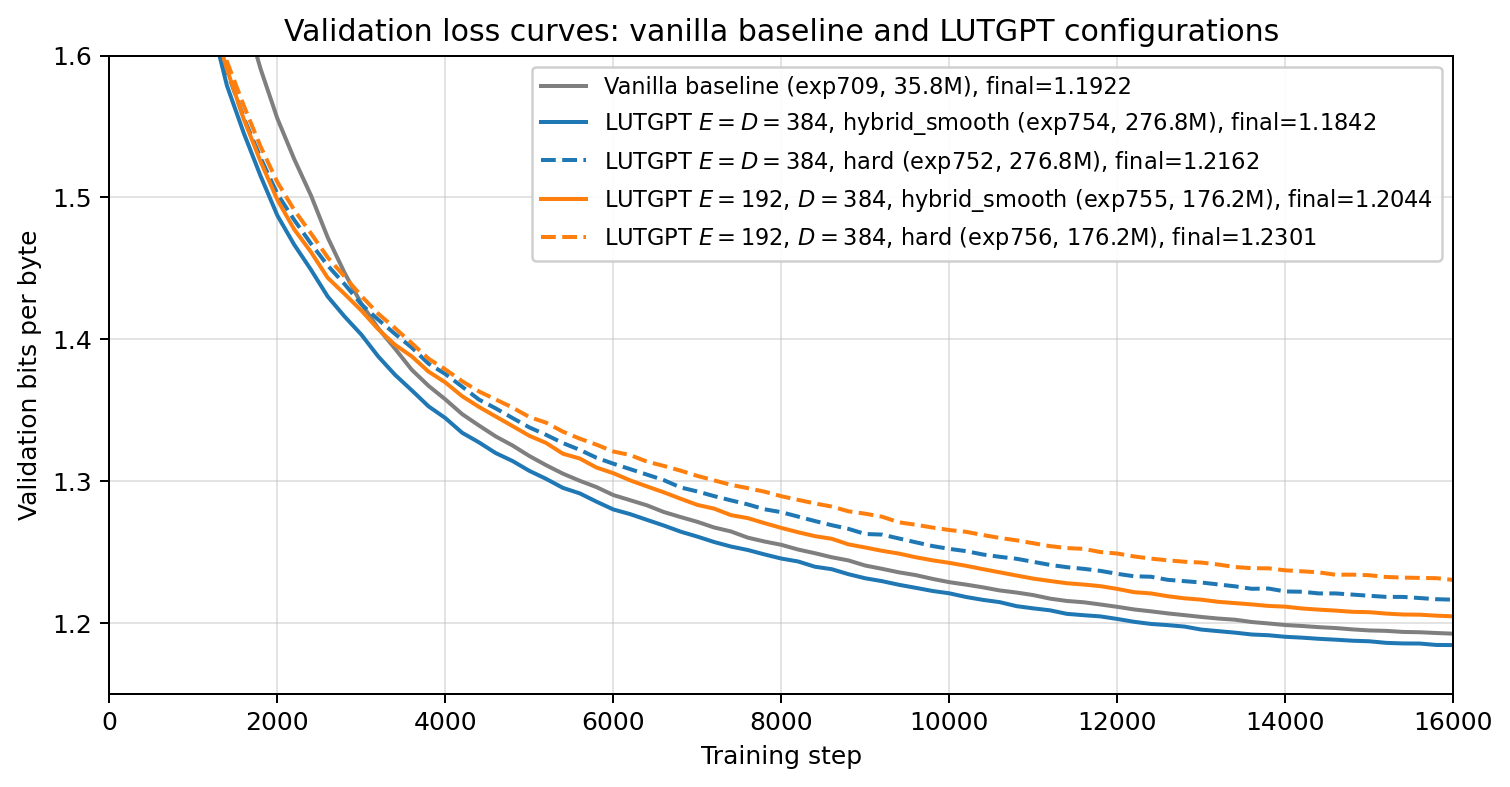
\includegraphics[width=0.78\linewidth,height=0.72\textheight,keepaspectratio]{figs/val_curves.png}

\smallskip
\scriptsize
Solid = \texttt{hybrid\_smooth}, dashed = \texttt{hard}. Grey = vanilla \texttt{exp709}; blue = full-width LUTGPT pair (\texttt{exp754}/\texttt{exp752}); orange = narrow-backbone pair (\texttt{exp755}/\texttt{exp756}). All five matched on training tokens. The hybrid-smooth curves sit slightly below their hard counterparts at every step.
\end{frame}

% =====================================================================
\begin{frame}{Loss curves --- wall-clock-matched hard training}
\centering
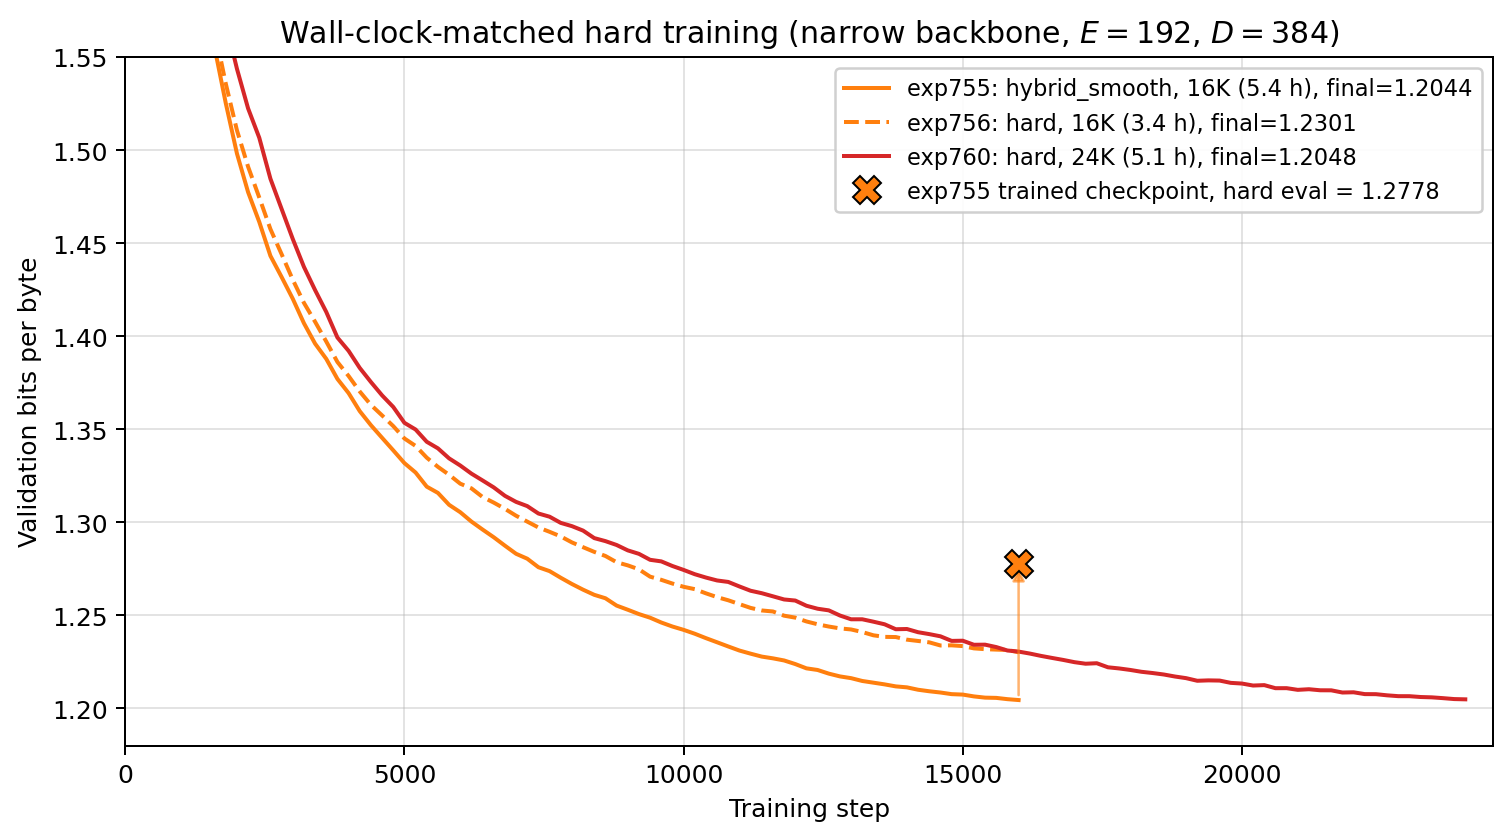
\includegraphics[width=0.78\linewidth,height=0.72\textheight,keepaspectratio]{figs/val_curves_wallclock.png}

\smallskip
\scriptsize
Same narrow backbone (\(E\!=\!192\), \(D\!=\!384\), \(176.2\,\)M). Hard is \(\sim\!1.6\times\) faster per step than hybrid-smooth, so \(1.5\times\) more hard steps fit in the same wall-clock budget. \texttt{exp760} (\(24\)K hard, \(5.1\)h) lands at \(1.2048\) --- inside noise of \texttt{exp755}'s \(1.2044\) at \(5.4\)h --- and ships in hard mode. The X marks the \(+73\) mb bump you'd pay by shipping the soft-trained checkpoint as hard.
\end{frame}

% =====================================================================
\begin{frame}{Loss curves --- halving the table count, doubling the tokens}
\centering
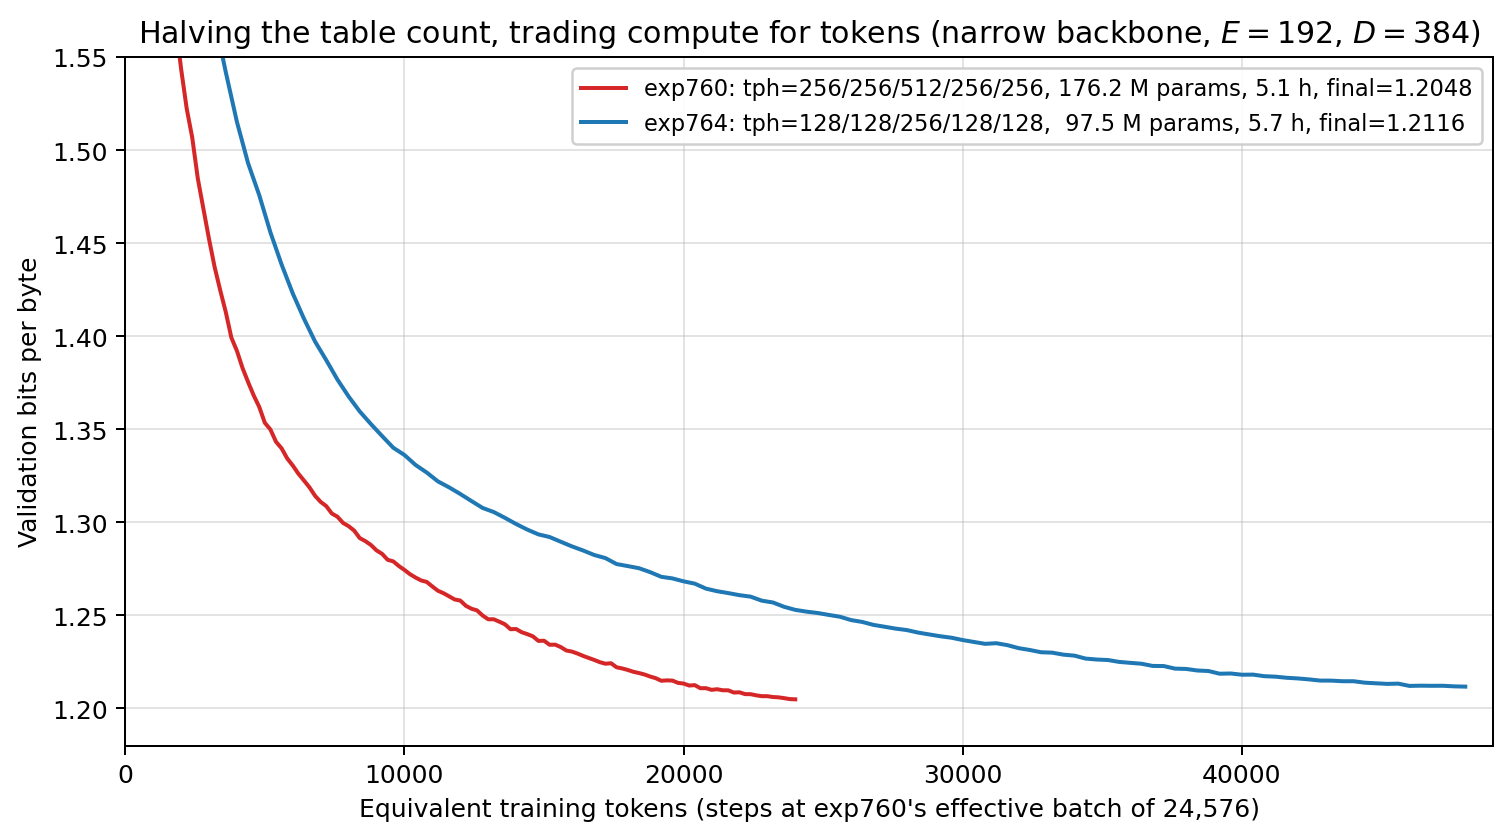
\includegraphics[width=0.78\linewidth,height=0.72\textheight,keepaspectratio]{figs/val_curves_tph_halved.png}

\smallskip
\scriptsize
\texttt{exp764} halves \(\mathrm{tph}\) at every LUT call site (\(176.2\,\)M \(\to\) \(97.5\,\)M, half the per-LUT HBM bandwidth) and spends the saved per-step compute on a \(2\times\) larger batch. The x-axis is rescaled so both runs are at matched training tokens; \texttt{exp764}'s \(24\)K steps plot as \(48\)K equivalent steps at \texttt{exp760}'s batch. The smaller model sits a few mb above at every matched-token point; final gap is \(+6.8\) mb.
\end{frame}

% =====================================================================
\appendix

\begin{frame}{Appendix --- soft-surrogate backward, derived (1/2)}
\small
\textbf{Setup} (per table). \;
Soft sign \(p_j = d_j/(\Tsoft + |d_j|) \in (-1, +1)\) with \(d_j = x_{a_j} - x_{b_j}\); bit parity \(\chi_j(b) = 2 b_j - 1\); row score and softmax over all \(K = 2^N\) rows:
\[ \mathcal{S}(b) = \sum_{j=1}^{N} p_j\, \chi_j(b), \qquad \pi(b) = \softmax_b\,\bigl(\mathcal{S}(b)/\Tsel\bigr). \]

\textbf{Synthetic full-K forward} (never computed at runtime; only used to define the input + temperature gradient):
\[ y_{\mathrm{full}} = \sum_b \pi(b)\, W[b]. \]
We backprop \(\partial L / \partial x\) and \(\partial L / \partial T\) \emph{as if} the forward had been \(y_{\mathrm{full}}\), regardless of the actual forward mode.

\textbf{Weight gradient} stays honest (only the rows actually visited):
\[
\frac{\partial L}{\partial W[r]} =
\begin{cases}
g\, [r = \bstar] & \text{hard,}\\
(1{-}u)\, g\, [r = \bstar] + u\, g\, [r = b_{\mathrm{alt}}] & \text{hybrid\_smooth.}
\end{cases}
\]
\end{frame}

\begin{frame}{Appendix --- soft-surrogate backward, derived (2/2)}
Let \(g = \partial L / \partial y \in \R^{\dout}\). Chain rule through the synthetic full-K forward:

\smallskip
\small
\textbf{Softmax} (gives \(g_z(b)\) per row score):
\[
g_\pi(b) = g^{\top} W[b], \quad
g_z(b) = \pi(b)\bigl(g_\pi(b) - \textstyle\sum_{b'} \pi(b')\, g_\pi(b')\bigr), \quad
g_{\mathcal S}(b) = g_z(b) / \Tsel.
\]

\textbf{Linear score} \(\mathcal{S}(b) = \sum_j p_j\, \chi_j(b)\), \textbf{soft sign} \(p_j = d_j/(\Tsoft + |d_j|)\):
\[
g_{p_j} = \sum_b g_{\mathcal S}(b)\, \chi_j(b), \qquad
g_{d_j} = g_{p_j}\,\Tsoft / (\Tsoft + |d_j|)^{2}.
\]

\textbf{Anchor-pair difference} \(d_j = x_{a_j} - x_{b_j}\), sparse-linear \(\Rightarrow\) scatter-add on \(x\); analogous derivations give \(\partial L/\partial \log \Tsel = -\sum_b g_z(b)\, z(b)\), \(\partial L/\partial \log \Tsoft = -\sum_j g_{d_j}\, d_j.\)
\end{frame}

\end{document}
